\documentclass[ngerman]{beamer}
\usepackage{etex}
\usepackage[beamer]{mydefs}
\usepackage{calc}
\usepackage{babel}
\usepackage{fontspec}
\usepackage{textpos}
%\usepackage{pgfplots}
\usepackage{pifont,stmaryrd}

%%%

\title{Lernen Terminologischen Wissens\\ mit hoher Konfidenz aus fehlerhaften Daten}
\author{Daniel Borchmann}
\date{9.\,September 2014}

%%%

%\includeonlyframes{current}
\usetikzlibrary{decorations.pathmorphing,calc,arrows}
\tikzset{>={stealth'[sep]}}

% \let\oldemph\emph
% \renewcommand{\emph}[1]{\alert<.>{\oldemph{#1}}}

\newcommand{\pseudocite}[1]{\textcolor{gray}{[#1]}}

%%%

\begin{document}

\begin{frame}[plain]
  \maketitle
\end{frame}

\begin{frame}

  \onslide<1->

  \begin{block}{Ziel}
    Wissen aus Daten für maschinelle Bearbeitung extrahieren
  \end{block}

  \onslide<2->

  \begin{block}{Beobachtung}
    \begin{itemize}
    \item<3-> faktisches Wissen leicht extrahierbar
    \item<8-> terminologisches (begriffliches) Wissen schwer extrahierbar
    \end{itemize}
  \end{block}

  \onslide<4->

  \vspace*{-0.6\baselineskip}
  \begin{overlayarea}{\linewidth}{13ex}
    \only<4-6>{
      \begin{Beispiel}[DBpedia/Wikidata]
        \only<5->{
          \begin{center}\ttfamily
            <http://dbpedia.org/resource/\alert<6->{Aldous\_Huxley}>\\
            <http://dbpedia.org/ontology/\alert<6->{notableWork}>\\
            <http://dbpedia.org/resource/\alert<6->{Brave\_New\_World}> .
          \end{center}
        }
      \end{Beispiel}
    }
    
    \only<9->{
      \begin{Beispiel}
        \begin{itemize}
        \item<10-> Jede Katze ist ein Säugetier.
        \item<11-> Hunde sind keine Katzen.
        \item<12-> Jeder Mensch, der ein Kind hat, ist ein Elternteil.
        \end{itemize}
      \end{Beispiel}
    }
  \end{overlayarea}

\end{frame}

\begin{frame}

  \onslide<1->
  
  \begin{block}{Grundlegende Fragen}
    \begin{itemize}
    \item<2-> Wie Wissen darstellen? \visible<5->{$\quad\Rightarrow\quad$
        \emph{Beschreibungslogiken} }
    \item<3-> Wie Wissen extrahieren? \visible<10->{$\quad\Rightarrow\quad$ \emph{Formale
          Begriffsanalyse}}
    \item<4-> Welches Wissen extrahieren? \visible<11->{$\quad\Rightarrow\quad$
        \emph{\enquote{interessantes}}}
    \end{itemize}
  \end{block}

  \onslide<6->

  \begin{Beispiel}[General Concept Inclusions, GCIs]
    \begin{itemize}
    \item<7-> $\mathsf{Cat} \sqsubseteq \mathsf{Mammal}$
    \item<8-> $\mathsf{Dog} \sqcap \mathsf{Cat} \sqsubseteq \bot$
    \item<9-> $\exists \mathsf{child}. \top \sqsubseteq \mathsf{Parent}$
    \end{itemize}
  \end{Beispiel}

\end{frame}

\begin{frame}

  \onslide<+->
  
  \centering
  
  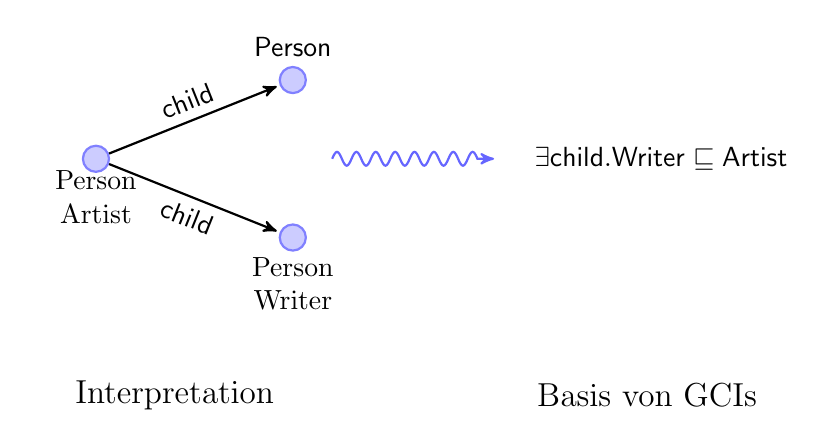
\begin{tikzpicture}[element/.style = {circle,draw=blue!50,fill=blue!20,thick}]
    \node[element, draw, circle, label=below:{\parbox{1.5cm}{\vspace*{-.5cm}\center
        Person\\Artist}}] (B) at (3,-1) {};
    \node[element, draw, circle, label=above:{\sf Person}] (C) at (5.5,0) {};
    \node[element, draw, circle, label=below:{\parbox{1.5cm}{\vspace*{-.4cm}\center
        Person\\Writer}}] (D) at (5.5,-2) {};
    \path[->,thick]
    (B) edge node[midway,above,sloped] {\sf child} (C)
    (B) edge node[midway,below,sloped] {\sf child} (D)
    ;

    \node[coordinate] (D) at (6,-1) {};

    \onslide<+->{
      \node  (E) at (10,-1) {$\quad\mathsf{\exists child.Writer} \sqsubseteq \mathsf{Artist}$};
      \draw[->,thick,blue!60,opaque=50,decorate,decoration={coil,aspect=0,post length=0.7em,
        segment length=0.7em}] (D) to (E);
    }

    \onslide<+->{
      \node at (4, -4) {\large Interpretation};
    }

    \onslide<+->{
      \node at (10, -4) {\large Basis von GCIs};
    }
  \end{tikzpicture}
  
\end{frame}

\begin{frame}

  \onslide<+->

  Fixiere disjunkte Mengen $N_{C}$ (Konzeptnamen) und $N_{R}$ (Rollennamen).

  \onslide<+->

  \begin{Definition}
    \emph{$\ELbot$-Konzeptbeschreibungen} $C$ sind von der Form
    \begin{equation*}
      C ::= A \mid C \sqcap\! C \mid \exists r. C \mid \bot \mid \top
    \end{equation*}
    für $A \in N_C, r \in N_R$.
  \end{Definition}

  \onslide<+->

  \begin{Beispiel}
    \begin{equation*}
      \mathsf{Cat} \sqcap \mathsf{Dog}, \exists \mathsf{child}. \mathsf{Writer}, \top, \bot
    \end{equation*}
  \end{Beispiel}

\end{frame}

\begin{frame}

  \onslide<+->
  \onslide<+->

  \begin{Definition}
    Eine \emph{Interpretation} $\mathcal{I} = (\Delta^{\mathcal{I}}, \cdot^{\mathcal{I}})$
    besteht aus
    \begin{itemize}
    \item<+-> einer nicht-leeren Menge $\Delta^{\mathcal{I}}$ von \emph{Elementen},
    \item<+-> einer Abbildung $\cdot^{\mathcal{I}}$ mit
      \begin{align*}
        A^{\mathcal{I}} &\subseteq \Delta^{\mathcal{I}} \\
        r^{\mathcal{I}} &\subseteq \Delta^{\mathcal{I}} \times \Delta^{\mathcal{I}}
      \end{align*}
      für $A \in N_{C}, r \in N_{R}$.
    \end{itemize}
  \end{Definition}

  \onslide<+->

  \begin{Definition}
    Für $A \in N_C$, $C, D$ zwei $\ELbot$-Konzeptbeschreibungen und $r \in N_R$ sei
    \begin{itemize}
    \item $\bot^{\mathcal{I}} = \emptyset$, $\top^{\mathcal{I}} = \Delta^{\mathcal{I}}$,
    \item $(C \sqcap D)^{\mathcal{I}} := C^{\mathcal{I}} \cap D^{\mathcal{I}}$,
    \item $(\exists r. C)^{\mathcal{I}} := \set{ x \in \Delta^{\mathcal{I}} \mid \exists y
        \in \Delta^{\mathcal{I}} \st (x, y) \in r^{\mathcal{I}}, y \in C^{\mathcal{I}} }$.
    \end{itemize}
  \end{Definition}

\end{frame}

\begin{frame}

  \onslide<+->

  \begin{Definition}
    Sind $C, D$ zwei $\ELbot$-Konzeptbeschreibungen, so heißt
    \begin{equation*}
      C \sqsubseteq D
    \end{equation*}
    \emph{Allgemeine Konzeptinklusion} (General Concept Inclusion, GCI).

    \onslide<+->%
    \medskip{}
    $C \sqsubseteq D$ \emph{gilt} in $\mathcal{I}$ falls
    \begin{equation*}
      C^{\mathcal{I}} \subseteq D^{\mathcal{I}}.
    \end{equation*}
  \end{Definition}

\end{frame}

\begin{frame}

  \onslide<+->
  
  \begin{Definition}
    $\con K = (G, M, I\,)$ heißt \emph{formaler Kontext}, falls $G, M$ Mengen und $I
    \subseteq G \times M$.

    \onslide<+->\medskip

    Für $A \subseteq G, B \subseteq M$ sei
    \begin{align*}
      \onslide<+->{A' &= \set{ m \in M \mid \forall g \in A \holds (g, m) \in I },} \\
      \onslide<+->{B' &= \set{ g \in G \mid \forall m \in B \holds (g, m) \in I }}.
    \end{align*}
  \end{Definition}
  
  \onslide<+->

  \begin{Definition}
    $A \to B$ heißt \emph{Implikation} in $\con K$, falls $A, B \subseteq M$. \onslide<+->
    $A \to B$ heißt \emph{gültig} in $\con K$, falls
    \begin{equation*}
      A' \subseteq B'.
    \end{equation*}
  \end{Definition}
  
\end{frame}

\begin{frame}

  \onslide<+->

  \begin{block}{Offene Frage}
    Was ist \enquote{interessantes} Wissen?
  \end{block}

  \onslide<+->

  \begin{block}{Erste Idee \pseudocite{Baader, Distel 2009}}
    \onslide<+->
    Betrachte alle \emph{gültigen} GCIs \onslide<+-> $\Longrightarrow$ berechne
    \emph{Basis} aller gültigen GCIs.
  \end{block}

  \onslide<+->

  \begin{block}{Beobachtung}
    \begin{itemize}
    \item<+-> GCIs sind Implikationen sehr ähnlich
    \item<+-> FBA bietet Möglichkeiten, Implikationen aus Daten zu berechnen
    \end{itemize}
    \onslide<+->%
    $\Longrightarrow$ FBA-Methoden verallgemeinern
  \end{block}

\end{frame}

\newcommand{\datacloud}{
  \begin{scope}[every node/.style={coordinate},scale=.4]
    \node (A) at (0,0) {};
    \node (B) at (2,3) {};
    \node (C) at (4,5) {};
    \node (D) at (6,3) {};
    \node (E) at (7,1) {};
    \node (F) at (5,-1) {};
    \node (G) at (3,-1.5) {};
    \node (H) at (2,-1) {};
    \draw [every edge/.style={bend left}, every to/.style={bend left=70}]
    (A) to (B) to (C) to (D) to (E) to (F) to (G) to (H) to (A);
  \end{scope}
}

\newcommand{\zoomindata}{
  \begin{scope}[scale=.6]
    \node[circle,draw,blue] (small circle) at (0,0) [minimum size=1cm] {};
    \node[circle,blue] (large circle) at (8,0) [minimum size=3.8cm] {};
    \draw[blue]
      let \p1 = (tangent cs:node={large circle},point={(0,0)},solution=2),
          \p2 = (tangent cs:node={large circle},point={(0,0)},solution=1),
          \p3 = (101:.83cm),
          \p4 = (-101:.83cm)
      in ($(small circle) + (\p3)$) -- ($(\p1) + (\p3)$)
         ($(small circle) + (\p4)$) -- ($(\p2) + (\p4)$);

    \begin{scope}[shift={(3,1)}]
      \path[clip] (5,-1) circle (4cm);
      \draw[line width=.1em,blue] (5,-1) circle (4cm);
      \node[coordinate] (A) at (0,0) {};
      \node[draw, circle, label=below:{\parbox{1.5cm}{\vspace*{-.5cm}\center
          Person\\Artist}}] (B) at (3,-1) {};
      \node[draw, circle, label=above:{\sf Person}] (C) at (7,0) {};
      \node[draw, circle, label=below:{\parbox{1.5cm}{\vspace*{-.4cm}\center
          Person\\Writer}}] (D) at (7,-2) {};
      \node[coordinate] (E) at (9.2,.5) {};
      \node[coordinate] (F) at (9.3,-2.3) {};
      \path[->,thick]
      (A) edge[lightgray] (B)
      (B) edge node[midway,above,sloped] {\sf child} (C)
      (B) edge node[midway,below,sloped] {\sf child} (D)
      (C) edge[lightgray] (E)
      (D) edge[lightgray] (F)
      ;
    \end{scope}
  \end{scope}
}

\begin{frame}

  \onslide<+->
  
  \begin{center}
    \vspace*{-3ex}
    \hspace*{-2ex}
    \begin{tikzpicture}
      \begin{scope}
        \datacloud;
      \end{scope}
      \onslide<2-3>{
        \begin{scope}[shift={(1.5,0.7)}]
          \zoomindata
        \end{scope}
      }

      \onslide<3->{
        \node[rectangle] (example gci) at (1.5,-3) {
          \makebox[3cm][r]{$\{\,\exists\mathsf{child}. \mathsf{Writer} \sqsubseteq
            \mathsf{Artist},\ldots\,\}$}};
        \draw[very thick] {
          (1.5,-1) edge[->, gray!90] node[left, black]
            {\parbox{3.5cm}{
                \vspace*{-.7cm}
                \center
                Basis gültiger GCIs
              }
            }
          (example gci)
        };
      }
      \onslide<5-> {
        \node at (1.5,3) {\makebox[0cm]{\emph{Beschreibungslogik}}};
        \node at (7,3) {\makebox[0cm]{\emph{Formale Begriffsanalyse}}};
        \draw[draw opacity=0.5] {
          ($ (current bounding box.north) + (1cm,0) $)
          -- ($ (current bounding box.south) + (1cm,0) $)
        };
      }
      \onslide<6-> {
        \node at (0,2) {$\mathcal{I}$};
        \node[rectangle] (induced context) at (7,.7) {
          \parbox{3cm}{
            \begin{equation*}
              \begin{array}{c|ccc}
                \con K_{\mathcal{I}} & & M_{\mathcal{I}} & \\
                \midrule
                & \times & \times & . \\
                \smash{\Delta^{\mathcal{I}}} & \times & . & \times \\
                & . & . & \times
              \end{array}
            \end{equation*}
          }
        };
        \draw[very thick,->, gray!90] (3.3,.7) to (induced context);
      }
      \onslide<7-> {
        \node[rectangle] (base of induced context) at (7,-3) {
          $\set{ U \to V \mid \ldots }$
        };
        \draw {
          (induced context) edge[very thick, ->, gray!90]
          node[midway,right, black] {
            \parbox{3cm}{
              \vspace*{-.3cm}
              \center
              Basis gültiger Implikationen
            }
          }
          (base of induced context)
        };
      }
      \onslide<8-> {
        \draw[very thick,->, gray!90] {
          (base of induced context) -- (example gci)
        };
      }
    \end{tikzpicture}
  \end{center}
  
\end{frame}

\begin{frame}

  \onslide<+->
  
  \begin{block}{Experiment \pseudocite{Borchmann, Distel 2011}}
    \begin{itemize}
    \item<+-> DBpedia: aus der Wikipedia halbautomatisch gewonnenes Wissen
    \item<+-> betrachte nur \textsf{child}-Relation ${} \leadsto \Idbpedia$
    \item<+-> $\Delta^{\Idbpedia} = 5626$
    \end{itemize}
  \end{block}

  \onslide<+->

  \begin{block}{Einige Ergebnisse}
    \vspace*{-3ex}
    \begin{gather*}
      \onslide<+->{\sf MemberOfParliament \sqsubseteq Person \sqcap Politician}~\\
      \onslide<+->{\sf \exists child. Person \sqsubseteq Person}~\\
      \onslide<+->{\sf FictionalCharacter \sqcap \exists child. Person \sqsubseteq \exists
        child. FictionalCharacter}
    \end{gather*}
  \end{block}

  \onslide<+->

  \begin{block}{Fragwürdige Ergebnisse}
    \vspace*{-3ex}
    \begin{gather*}
      \onslide<+->{\sf Person \sqcap \exists child. Book \sqsubseteq
        FictionalCharacter}~\\
      \onslide<+->{\sf Criminal \sqcap \exists child. Politician \sqsubseteq \bot}~\\
      \onslide<+->{\sf Person \sqcap \exists child. Criminal \sqsubseteq Criminal}
    \end{gather*}
  \end{block}

\end{frame}

\begin{frame}
  
  \onslide<1-8>

  \begin{block}{Beobachtung}
    \begin{equation*}
      \sf \exists child. \top \sqsubseteq Person
    \end{equation*}
    \onslide<2->%
    \emph{gilt nicht} in $\Idbpedia$\onslide<3->, denn es gibt 4 \alt<7->{\alert{falsche
        Gegenbeispiele:}}{Gegenbeispiele, d.\,h.}
    \begin{overlayarea}{\textwidth}{5ex}
      \only<4-6>{
        \begin{equation*}
          \abs{ (\sf \exists child.\top)^{\Idbpedia} \setminus Person^{\Idbpedia} } = 4.
        \end{equation*}
      }
      \only<8->{
        \begin{equation*}
          \text{\texttt{Teresa\_Carpio}, \texttt{Charles\_Heung},
            \texttt{Adam\_Cheng}, \texttt{Lydia\_Shum}.}
        \end{equation*}
      }
    \end{overlayarea}

    \onslide<5->

    \bigskip{}

    Andererseits: 2547 Elemente in $\Idbpedia$ erfüllen $\sf \exists child. \top
    \sqsubseteq \sf Person$, d.\,h.
    \begin{equation*}
      \abs{ (\sf \exists child.\top \sqcap Person)^{\Idbpedia} } = 2547.
    \end{equation*}

    \onslide<6->

    $\sf \exists child. \top \sqsubseteq Person$ ist also
    \alt<7->{\alert{\enquote{\sout{fast}}}}{\enquote{\makebox[\widthof{\sout{fast}}]{fast}}} richtig.
  \end{block}

\end{frame}

\begin{frame}

  \onslide<+->

  \begin{block}{Intuition}
    Betrachte auch GCIs, die \enquote{fast} richtig sind.
  \end{block}

  \onslide<+->
  \begin{Definition}
    Die \emph{Konfidenz} von $C \sqsubseteq D$ in $\mathcal{I}$ ist gegeben durch
    \begin{equation*}
      \conf_{\mathcal{I}}(C \sqsubseteq D) :=
      \begin{cases}
        1, & \text{falls } C^{\mathcal{I}} = \emptyset,\\
        \frac{\abs{(C \sqcap D)^{\mathcal{I}}}}{\abs{C^{\mathcal{I}}}} & \text{sonst}.
      \end{cases}
    \end{equation*}
    \onslide<+->%
    Sei $c \in [0, 1]$.  Dann
    \begin{equation*}
      \Th_c(\mathcal{I}) := \set{ C \sqsubseteq D \mid \conf_{\mathcal{I}}(C \sqsubseteq
        D) \ge c}.
    \end{equation*}
  \end{Definition}

  \onslide<+->

  \begin{block}{Ansatz \pseudocite{Borchmann 2012}}
    Betrachte $\Th_{c}(\mathcal{I})$ als \enquote{interessantes} Wissen in $\mathcal{I}$.
  \end{block}

\end{frame}

\begin{frame}

  \onslide<+->

  \hbox{}\vfill{}
  
  \begin{center}
    \hspace*{-2ex}
    \begin{tikzpicture}
      \begin{scope}
        \datacloud;
      \end{scope}

      \node[rectangle] (example gci) at (1.5,-3) {
        \makebox[3cm][r]{$\{\,\exists\mathsf{child}. \mathsf{Writer} \sqsubseteq
          \mathsf{Artist},\ldots\,\}$}};
      \draw[very thick] {
        (1.5,-1) edge[->, gray!90] node[left, black]
          {\parbox{3.5cm}{
              \vspace*{-.7cm}
              \center
              \alt<2->{\parbox{4cm}{\raggedright Basis von GCIs\\mit \alert{hoher
                    Konfidenz}}}{Basis gültiger GCIs}
            }
          }
        (example gci)
      };

      \node at (0,2) {$\mathcal{I}$};
      \node[rectangle] (induced context) at (7,.7) {
        \parbox{3cm}{
          \begin{equation*}
            \begin{array}{c|ccc}
              \con K_{\mathcal{I}} & & M_{\mathcal{I}} & \\
              \midrule
              & \times & \times & . \\
              \smash{\Delta^{\mathcal{I}}} & \times & . & \times \\
              & . & . & \times
            \end{array}
          \end{equation*}
        }
      };
      \draw[very thick,->, gray!90] (3.3,.7) to (induced context);

      \node[rectangle] (base of induced context) at (7,-3) {
        $\set{ U \to V \mid \ldots }$
      };
      \draw {
        (induced context) edge[very thick, ->, gray!90]
        node[midway,right, black] {
          \parbox{3cm}{
            \vspace*{-.3cm}
            \center
            \alt<3->{\parbox{2.9cm}{\raggedright Basis von Implikationen mit \\\alert{hoher
                  Konfidenz}}}{Basis gültiger Implikationen}
          }
        } (base of induced context) };

      \draw[very thick,->, gray!90] {
        (base of induced context) -- (example gci)
      };
    \end{tikzpicture}
  \end{center}

  \vfill
  \hbox{}

\end{frame}

\begin{frame}

  \onslide<+->

  \begin{block}{Parallelen zwischen FBA und BL}
    \begin{center}
      \begin{tabular}{c|c}
        Formale Begriffsanalyse & Beschreibungslogik \\
        \midrule\onslide<+->
        Gegenstände $G$ & Elemente $\Delta^{\mathcal{I}}$ \\\onslide<+->
        Merkmale $M$ & Konzeptbeschreibungen \\\onslide<+->
        Formale Kontexte $\con K$ & Interpretationen $\mathcal{I}$ \\\onslide<+->
        Implikationen & GCIs \\\onslide<+->
        $A', A \subseteq M$ & $(\bigsqcap A)^{\mathcal{I}}$ \\\onslide<+->
        $B', B \subseteq G$ & \textcolor{red}{\textbf{?}}
      \end{tabular}
    \end{center}
  \end{block}

  \onslide<+->

  \begin{block}{Definition \pseudocite{Baader, Distel 2009}}
    Sei $X \subseteq \Delta^{\mathcal{I}}$. \onslide<+-> Eine Konzeptbeschreibung $C$
    heißt \emph{model-based most-specific concept description} von $X$ in $\mathcal{I}$
    falls
    \begin{itemize}
    \item<+-> $X \subseteq C^{\mathcal{I}}$ und
    \item<+-> für jedes $D$ mit $X \subseteq D^{\mathcal{I}}$ ist $C$ \emph{spezieller
        als} $D$.
    \end{itemize}
    \onslide<+->%
    Bezeichnung: $C = X^{\mathcal{I}}$
  \end{block}

\end{frame}

% \begin{frame}

%   \onslide<1->

%   \begin{block}{Problem}
%     Existenz von model-based most-specific concept descriptions in \ELbot\ nicht gesichert
%   \end{block}

%   \onslide<2->
  
%   \begin{block}{Auswege}
%     \begin{itemize}
%     \item<3-> Rollentiefe beschränken \pseudocite{[Distel 2012]}
%     \item<4-> \alert<5->{Logik erweitern} \pseudocite{[Baader, Distel 2009]} \onslide<6->
%       $\leadsto$ \ELgfpbot \pseudocite{[Nebel 1991, Baader 2002/2003]}
%     \end{itemize}
%   \end{block}

% \end{frame}

\begin{frame}

  \onslide<+->

  \begin{Definition}
    \begin{equation*}
      M_{\mathcal{I}} = N_{C} \cup \set{ \bot } \cup \set{ \exists r. X^{\mathcal{I}} \mid
        X \subseteq \Delta^{\mathcal{I}}, X \neq \emptyset }.
    \end{equation*}
  \end{Definition}

  \onslide<+->

  \begin{Definition}
    Setze $\con K_{\mathcal{I}} = (\Delta^{\mathcal{I}}, M_{\mathcal{I}}, \nabla)$ mit
    \begin{equation*}
      (x, C) \in \nabla \iff x \in C^{\mathcal{I}}.
    \end{equation*}
  \end{Definition}

  \onslide<+->

  \begin{block}{Satz \pseudocite{Baader, Distel 2009}}
    Ist $\mathcal{L}$ eine Basis von $\con K_{\mathcal{I}}$, dann ist
    \begin{equation*}
      \set{ \bigsqcap U \sqsubseteq (\bigsqcap U)^{\mathcal{I}\mathcal{I}} \mid (U \to V)
        \in \mathcal{L} }
    \end{equation*}
    eine Basis von $\mathcal{I}$.    
  \end{block}
  
\end{frame}

\begin{frame}

  \onslide<+->

  \begin{block}{Problem}
    Wie Basen von $\Th_{c}(\mathcal{I})$ finden?
  \end{block}

  \onslide<+->

  \begin{block}{Ansatz \pseudocite{Luxenburger 1993, Borchmann 2012}}
    \begin{itemize}
    \item<+-> Finde Basen von $\Th_{c}(\mathcal{I}) \setminus \Th(\mathcal{I})$.
    \item<+-> Betrachte nur Konzeptbeschreibungen der Form $(C^{\mathcal{I}})^{\mathcal{I}}$.
    \end{itemize}
  \end{block}

  % \onslide<+->
  
  % \begin{block}{Die Idee in FBA}
  %   \onslide<+->%
  %   Es sei $\mathcal{B}$ Basis von $\con K$,
  %   \begin{equation*}
  %     \mathcal{C} = \set{ X'' \to Y'' \mid 1 > \conf_{\con K}(X'' \to Y'') \ge c }
  %   \end{equation*}
  %   und $1 > \conf(A \to B) \ge c$.  \onslide<+-> Dann $\conf_{\con K}(A \to B) =
  %   \conf_{\con K}(A'' \to B'')$ \onslide<+-> und
  %   \begin{equation*}
  %     \mathcal{B} \cup \mathcal{C} \models A \to A'' \onslide<+-> \to B'' \onslide<+->
  %     \to B.
  %   \end{equation*}
  % \end{block}

  \onslide<+->

  \begin{Definition}
    \begin{equation*}
      \Conf(\mathcal{I}, c) := \set{ X^{\mathcal{I}} \sqsubseteq Y^{\mathcal{I}} \mid Y
        \subseteq X \subseteq \Delta_{\mathcal{I}}, 1 > \conf_{\mathcal{I}}(
        X^{\mathcal{I}} \sqsubseteq Y^{\mathcal{I}}) \ge c}.
    \end{equation*}
  \end{Definition}

  \onslide<+->

  \begin{block}{Satz \pseudocite{Borchmann 2012}}
    Es sei $\mathcal{B}$ eine endliche Basis von $\mathcal{I}$, und $c \in [0, 1]$.  Dann
    ist 
    \begin{equation*}
      \mathcal{B} \cup \Conf(\mathcal{I},c)
    \end{equation*}
    eine endliche Basis $\Th_c(\mathcal{I})$.
  \end{block}
  
\end{frame}

\begin{frame}

  \onslide<1->
  
  \def\greenmark{\qquad\textcolor{green!80!black}{\checkmark}}

  \begin{block}{Experiment}
    \onslide<2->
    \begin{align*}
      \Conf(\Idbpedia, 0.95) = \visible<3->{ \{\,
        & \sf \exists child. \top \sqsubseteq Person, \visible<4->{\greenmark}\\
        & \sf Place \sqsubseteq PopulatedPlace, \visible<6->{\greenmark}\\
        & \sf \exists child. \exists child. \top \sqcap \exists child. OfficeHolder
        \visible<13->{\qquad\textcolor{red}{\textbf{\ding{55}}}} \\
        & \sf \quad \sqsubseteq \exists child.(OfficeHolder \sqcap \exists child. \top) \,\}}
    \end{align*}
  \end{block}

  \begin{overlayarea}{\linewidth}{24ex}
    \only<5-6>{
      \begin{block}{Gegenbeispiel zu erster GCI}
        \begin{equation*}
          \sf Greenwich\_Village
        \end{equation*}
      \end{block}
    }
    \only<8->{
      \begin{block}{Gegenbeispiel zu dritter GCI}
        \begin{equation*}
          \sf Pierre\_Samuel\_du\_Pont\_de\_Nemours
        \end{equation*}
      \end{block}
      \only<9-13>{Zwei Kinder:
        \begin{itemize}
        \item<10-> \emph{Victor Marie du Pont}, Diplomat, 4 Kinder,
          \only<11->{\emph{aber keines davon ``berühmt''.}}
        \item<12-> \emph{Eleuthère Irénée du Pont}, Industrieller
        \end{itemize}
      }
    }

  \end{overlayarea}

\end{frame}

% \begin{frame}

%   \onslide<1->

%   \begin{center}
%     \begin{tikzpicture}
%       \begin{axis}[ymax=1500]
%         \addplot[blue, no marks] coordinates {
%           (0.00,    1)
%           (0.01,    1)
%           (0.02,    1)
%           (0.03,    1)
%           (0.04,    1)
%           (0.05,    1)
%           (0.06,    1)
%           (0.07,    1)
%           (0.08,    1)
%           (0.09,    1)
%           (0.10,    1)
%           (0.11,    1)
%           (0.12,    1)
%           (0.13,    1)
%           (0.14,    1)
%           (0.15,    1)
%           (0.16,    1)
%           (0.17,    1)
%           (0.18,    1)
%           (0.19,  114)
%           (0.20,  114)
%           (0.21,  128)
%           (0.22,  128)
%           (0.23,  128)
%           (0.24,  141)
%           (0.25,  154)
%           (0.26,  163)
%           (0.27,  212)
%           (0.28,  212)
%           (0.29,  212)
%           (0.30,  227)
%           (0.31,  227)
%           (0.32,  227)
%           (0.33,  227)
%           (0.34,  227)
%           (0.35,  227)
%           (0.36,  227)
%           (0.37,  246)
%           (0.38,  250)
%           (0.39,  250)
%           (0.40,  264)
%           (0.41,  264)
%           (0.42,  295)
%           (0.43,  319)
%           (0.44,  319)
%           (0.45,  319)
%           (0.46,  319)
%           (0.47,  335)
%           (0.48,  346)
%           (0.49,  357)
%           (0.50,  551)
%           (0.51,  551)
%           (0.52,  561)
%           (0.53,  561)
%           (0.54,  604)
%           (0.55,  604)
%           (0.56,  606)
%           (0.57,  606)
%           (0.58,  626)
%           (0.59,  632)
%           (0.60,  641)
%           (0.61,  641)
%           (0.62,  641)
%           (0.63,  645)
%           (0.64,  675)
%           (0.65,  688)
%           (0.66,  688)
%           (0.67,  772)
%           (0.68,  913)
%           (0.69,  943)
%           (0.70,  954)
%           (0.71,  970)
%           (0.72, 1014)
%           (0.73, 1036)
%           (0.74, 1040)
%           (0.75, 1099)
%           (0.76, 1099)
%           (0.77, 1110)
%           (0.78, 1110)
%           (0.79, 1110)
%           (0.80, 1139)
%           (0.81, 1142)
%           (0.82, 1144)
%           (0.83, 1145)
%           (0.84, 1167)
%           (0.85, 1171)
%           (0.86, 1192)
%           (0.87, 1192)
%           (0.88, 1216)
%           (0.89, 1216)
%           (0.90, 1239)
%           (0.91, 1240)
%           (0.92, 1240)
%           (0.93, 1242)
%           (0.94, 1242)
%           (0.95, 1241)
%           (0.96, 1241)
%           (0.97, 1245)
%           (0.98, 1245)
%           (0.99, 1245)
%           (1.00, 1252)
%         };
%         \addlegendentry{$\abs{\Can(\Th_c(\con{K}_\Idbpedia))}$}
%       \end{axis}
%       \node (A) at (4.3,3.2) {};
%       \node (B) at (3.4,1.8) {};
%       \node (C) at (1.7,0.7) {};
%       \visible<5->{\node (A1) at (7,-1)  {$\sf \emptyset \to \set{Person}$};}
%       \visible<4->{\node (B1) at (3,-1)  {$\sf \set{\exists child.\top} \to \set{\exists
%             child. Person}$};}
%       \visible<3->{\node (C1) at (-1,-1) {$\sf \emptyset \to M_{\mathcal{I}}$};}
%       \onslide<2->{
%         \draw[red,very thick,->] {
%           (A1) edge (A)
%           (B1) edge (B)
%           (C1) edge (C)
%         };
%       }
%     \end{tikzpicture}
%   \end{center}

% \end{frame}

\begin{frame}

  \onslide<+->

  \begin{block}{Problem}
    Ansatz kann \emph{fehlerhafte Daten} von \emph{seltenen Gegenbeispielen} nicht
    unterscheiden.
  \end{block}

  \onslide<+->

  \begin{Beispiel}
    Die Aussage \emph{Alle Säugetieren gebären lebend},
    \begin{equation*}
      \mathsf{Mammal} \sqsubseteq \mathsf{LiveBearing},
    \end{equation*}
    \onslide<+->
    hat Gegenbeispiel \emph{Schnabeltier}.
  
    \begin{textblock*}{\linewidth}[0.5,0.5](0.85\linewidth,-1cm)
      \centering
      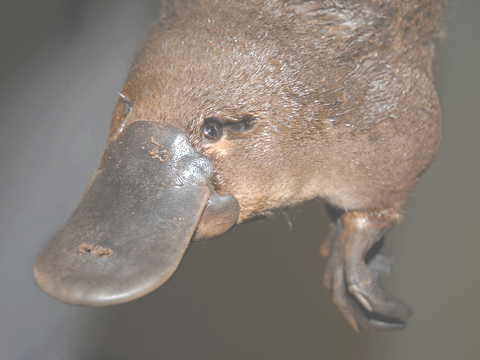
\includegraphics[width=3cm]{platypus}\\[-2ex]
      {\fontsize{3pt}{4pt}\selectfont http://www.sealifeconservation.org.au/adopt-an-animal/}
    \end{textblock*}

  \end{Beispiel}

  \onslide<+->

  \begin{block}{Ausweg}
    Verwendung externer \emph{Experten}%
    \onslide<+->%
    $\implies$ Merkmalexploration mit Implikationen/GCIs mit hoher Konfidenz
    \pseudocite{Borchmann 2013a, Borchmann 2013b}
  \end{block}

\end{frame}

% \begin{frame}

%   \onslide<+->

%   \begin{center}
%     \begin{tikzpicture}
%       \node[draw=blue!50,thick,rounded corners,fill=blue!30] (expert) at (-3,0) {Experte};
%       \begin{scope}
%         \node[draw=green!50,thick,rounded corners,fill=green!30] (algorithm) at (3,0) {Algorithmus};
%         \node (context) at (-1.5,-2.5) {
%           \parbox[t][15ex]{20ex}{
%             $\begin{array}[c]{c|ccc}
%               \con K & m_1 & \ldots & m_n \\
%               \midrule
%               g_1 & & \ldots & \\
%               \vdots & \\
%               g_k & & \ldots & \\
%               \visible<7>{
%                 \textcolor{red!70!black}{g_{k+1}}
%                 & &
%                 \makebox[3.5ex]{
%                   \textcolor{red!70!black}{
%                     \tikz[baseline]{\draw (0,0) edge node[pos=0.5,fill=white]{\ensuremath{C}} (2.2,0);}
%                   }
%                 }
%               }
%             \end{array}$
%           }
%         };
%         \node (knowledge) at (2,-2.5) {
%           \parbox[t][15ex]{10ex}{
%             $\begin{aligned}
%               \mathcal{S} = \{\, & A_1 \to B_1, \\ & \ldots \\ & A_\ell \to B_\ell
%               \alt<4>{, \\ & \textcolor{green!80!black}{X \to Y} \,\}}{\,\}}
%             \end{aligned}$
%           }
%         };
%       \end{scope}
%       %
%       \visible<2-7>{
%         \draw (algorithm) edge[->,thick,bend right=10] node[midway,above] {$X \to Y$
%           gültig?} (expert);
%       }
%       %
%       \visible<3-4>{
%         \draw (expert) edge[->,thick,bend right=10] node[midway,below]
%         {\textcolor{green!80!black}{Ja}} (algorithm);
%       }
%       %
%       \visible<6-7>{
%         \draw (expert) edge[->,thick,bend right=10] node[midway,below]
%         {\textcolor{red!70!black}{Nein}, Gegenbeispiel \textcolor{red!70!black}{$C$}} (algorithm);
%       }
%     \end{tikzpicture}
%   \end{center}

%   \onslide<9->

%   \vspace*{-4ex}
%   \begin{block}{Bemerkung}
%     \begin{itemize}
%     \item<10-> Nach Abschluss der Exploration gilt $\Cn(\mathcal{S}) = \Th(\con K)$ und
%       $\mathcal{S}$ ist eine Basis der vom Experten bestätigten Implikationen.
%     \item<11-> Die Anzahl der \emph{bestätigten} Implikationen ist kleinst-möglich.
%     \end{itemize}
%   \end{block}

%   \onslide<12->

%   \begin{block}{Resultat \pseudocite{Distel 2008}}
%     Merkmalexploration für gültige GCIs einer endlichen Interpretation möglich
%   \end{block}
  
% \end{frame}

% \begin{frame}

%   \onslide<1->

%   \begin{block}{Ziel}
%     Exploration auch für GCIs/Implikationen mit hoher Konfidenz
%   \end{block}

%   \onslide<2->
%   \begin{block}{Problem}
%     Erzeugung von Implikationen schwieriger
%   \end{block}

%   \vspace*{-0.6\baselineskip}
%   \begin{overlayarea}{\linewidth}{7\baselineskip}
%     \only<3-4>{
%       \begin{block}{Ursache}
%         Operator $\conf$ nicht monoton: \onslide<4->%
%         \begin{align*}
%           \conf(A \to B) &< c \\
%           \conf(C \to B) &\ge c
%         \end{align*}
%         für $C \subseteq A$ möglich.
%       \end{block}
%     }
    
%     \only<6->{
%       \begin{block}{Ausweg}
%         \begin{itemize}
%         \item<7-> Mehr Implikationen abfragen
%           \only<8-9>{
%             \begin{align*}
%               \onslide<8->{A &\to A'' \quad (\text{für abgeschlossene } A)} \\
%               \onslide<9->{B'' &\to \set{ m } \quad (\text{falls } \conf(B'' \to \set{m}) \ge
%                 c) }
%             \end{align*}
%           }
%         \item<11-> Bei GCIs: mehr Fragen an den Experten
%         \end{itemize}
%       \end{block}

%       \onslide<12->{
%         \begin{block}{Resultat \pseudocite{Borchmann 2013a, Borchmann 2013b}}
%           Merkmalexploration auch mit Implikationen/GCIs mit hoher Konfidenz möglich
%         \end{block}
%       }
%     }
%   \end{overlayarea}
  
% \end{frame}

\begin{frame}

  \onslide<+->

  \begin{block}{Zusammenfassung}
    \begin{itemize}
    \item<+-> Experimentelle Untersuchung der Resultate von Baader und Distel
    \item<+-> Erweiterung der Resultate um den Begriff der \emph{Konfidenz}
    \item<+-> Experimentelle Auswertung dieses Ansatzes
    \item<+-> Ausarbeitung einer Merkmalexploration von Implikationen/GCIs mit hoher
      Konfidenz
    \end{itemize}
  \end{block}

  \onslide<+->

  \begin{block}{Ausblick}
    \begin{itemize}
    \item<+-> Anwendung auf praktische Probleme (medizinische Daten)
    \item<+-> Adaption und Optimierung der entwickelten Algorithmen
    \item<+-> Beschränkte Rollentiefe \pseudocite{Distel 2012}
    \end{itemize}
  \end{block}
    
\end{frame}

\end{document}

%%% Local Variables: 
%%% mode: latex
%%% TeX-master: t
%%% ispell-local-dictionary: "de_DE"
%%% TeX-engine: luatex
%%% End: 

%  LocalWords:  Wikidata Concept Inclusions Konzeptnamen Rollennamen Konzeptinklusionen
%  LocalWords:  Ableitungsoperatoren Konzeptinklusion Inclusion label current node at of
%  LocalWords:  style opacity context induced base FBA model based most specific concept
%  LocalWords:  description descriptions LiveBearing
